%!TEX root = main.tex
	\section{Формализация игры. Ядро}
	
	\subsection{Тренировочные задачи}
	
	\task
	Имеется 5 продавцов и 3 покупателя. У каждого продавца есть по 1 товару. Все товары одинаковы. Каждый из покупателей хочет приобрести 1 единицу товара. Если $m$ продавцов и $n$ покупателей встречаются, то их полезность равна количеству проданных единиц товара, то есть $\min (m, n)$.
	
	Обозначим продавцов через $A,\,B,\,C,\,D,\,E$, а покупателей через $1,\,2,\,3$. Формализуем данную игру как коалиционную.
	
	Какие из приведенных ниже выигрышей коалиций заданы правильно?
	
	\solution
	Необходимо лишь проверить, что выигрыш в точности равен $v(m, n) = \min(m, n)$. Этому условию удовлетворяет два ответа:
	\begin{enumerate}[label=-]
		\item $v(A, B, 1, 2) = 2$
		\item $v(A, B, 1, 2, 3) = 2$
	\end{enumerate}
		
	\task
	Имеется 5 продавцов и 3 покупателя. У каждого продавца есть по 1 товару. Все товары одинаковы. Каждый из покупателей хочет приобрести 1 единицу товара. Если $m$ продавцов и $n$ покупателей встречаются, то их полезность равна количеству проданных единиц товара, то есть $\min(m,n)$.
	
	Обозначим продавцов через $A,\,B,\,C,\,D,\,E$, а покупателей через $1,\,2,\,3$. Формализуем данную игру как коалиционную.
	
	Рассмотрим ядро этой игры. Какие утверждения про ядро выполнены?
	
	\begin{enumerate}[label=$\circ$]
		\item Ядро пусто.
		\item Ядро состоит из единственного дележа: продавцы получают по 1/5, покупатели - по 2/3.
		\item[$\circledcirc$] Ядро состоит из единственного дележа: продавцы получают по 0, покупатели - по 1.
		\item Ядро состоит из всех платежей, в которых $x_1+x_2+x_3 = 3$ (здесь $x_i$ - платёж покупателя $i$).
	\end{enumerate}

	\solution
Выпишем условие на ядро. Имеется равенство $x_{A}+x_{B}+x_{C}+x_{D}+x_{E}+x_{1}+x_2+x_3=3$ и набор неравенств для всех коалиций. Заметим, что $x_A+x_B+x_C +x_1+x_2+x_3 \geq 3$, откуда $x_D+x_E=0$, а значит, $x_D=x_E=0$. Аналогично, $x_A=x_B=x_C=0$. Из неравенства $x_A+x_i\geq 1$ для любого $i$ получаем, что $x_1, x_2, x_3 \geq 1$, а так как их сумма равна 3, то $x_1=x_2=x_3=1$.

Легко проверить что данный делёж удовлетворяет всем неравенствам.
	
	\task
	Поменяем количество продавцов и покупателей в предыдущей задаче. Несложно понять, что такое же ядро будет и в игре $M$ продавцов и $N$ покупателей при $M \neq N$. Поймём что будет, если их количества совпадают. Рассмотрим следующую игру.
	
	Имеется 4 продавца и 4 покупателя. У каждого продавца есть по 1 товару. Все товары одинаковы. Каждый из покупателей хочет приобрести 1 единицу товара. Если mm продавцов и nn покупателей встречаются, то их полезность равна количеству проданных единиц товара, то есть $\min(m,n)$.
	
	Обозначим продавцов через $A,B,C,D$, а покупателей через $1,2,3,4$. Формализуем данную игру как коалиционную.
	
	Рассмотрим ядро этой игры. Какие дележи входят в ядро?
	
	\begin{enumerate}[label=$\circledcirc$]
		\item Всем продавцам - 0, всем покупателям - по 1.
		\item Всем продавцам - 1, всем покупателям - по 0.
		\item Всем игрокам по 1/2.
		\item Всем продавцам по 2/3, всем покупателям - по 1/3.
	\end{enumerate}

	\solution
	Выпишем условие на ядро. Имеется равенство $x_{A}+x_{B}+x_{C}+x_{D}+x_{1}+x_2+x_3+x_4=4$ и набор неравенств для всех коалиций. Заметим, что $x_{A}+x_1\geq 1$, $x_B+x_2 \geq 1$, $x_C+x_3\geq 1$, $x_D+x_4\geq 1$. Так как сумма переменных в правой части неравенств равна 4, мы получаем, что данные неравенства являются равенствами. Отсюда несложно получить, что $x_A=x_B=x_C=x_D=\alpha$, $x_1=x_2=x_3=x_4=1-\alpha$. При этом данные дележи удовлетворяют всем неравенствам.
	
	Следовательно, все дележи из условия подходят.

	\task
	\label{sec4}
	Трое жителей: Аркадий, Борис и Василий, живут в соседних домиках. У каждого из них есть предпочтение в каком из домиков жить (эти предпочтения заданы в виде полезности). Несколько жителей могут договориться поменяться домиками для максимизации суммарной полезности. Предположим, что полезности заданы в виде следующей таблицы (по строчкам жители, а по столбцам домики):
	
	\begin{table}[h]
		\label{prob4:table1}
		\caption{}
		\centering
		\begin{tabular}{|c|c|c|c|}
			\hline & А & Б & В \\ 	
			\hline Аркадий & 2 & 4 & 7 \\ 
			\hline Борис & 3 & 2 & 1 \\ 
			\hline Василий & 5 & 4 & 4 \\ 
			\hline 
		\end{tabular} 
	\end{table}
	
	Формализуем данную игру как коалиционную (занумеруем игроков в алфавитном порядке). Рассмотрим ядро данной игры.
	
	Отметьте верные неравенства, накладываемые на дележ $(x_1,x_2,x_3)$ из ядра игры (которые соответствуют условиям, накладываемым на коалиции).
	
	\begin{enumerate}[label=$\circ$]
		\item $x_1 \geq 7$
		\item[$\circledcirc$] $x_1 + x_2 \geq 7$
		\item[$\circledcirc$] $x_2 + x_3 \geq 6$
		\item $x_1 + x_3 \geq 11$
	\end{enumerate}

	\solution
	\label{arkadiy:sol1}
	Аркадий сам по себе не может поменять свой домик. Поэтому выигрыш коалиции $A$ равен стоимости домика для Аркадия, то есть $2$. Поэтому соответствующее неравенство должно выглядеть так: $x_1 \geq 2$.
	
	Рассмотрим Аркадия и Бориса. Если они не поменяются домиками, их суммарная полезность будет равна $2+2=4$, а если поменяются, то $4+3=7$. Отсюда выигрыш из коалиции составляет 7, и поэтому $x_1+x_2 \geq 7$.
	
	Рассмотрим Бориса и Василия. Если они не поменяются домиками, их суммарная полезность будет равна $2+4=6$, а если поменяются, то $1+4=5$. Отсюда выигрыш из коалиции составляет 6, и поэтому $x_2+x_3 \geq 6$.
	
	Рассмотрим Аркадия и Василия. Если они не поменяются домиками, их суммарная полезность будет равна $2+4=6$, а если поменяются, то $7+5=12$. Отсюда выигрыш из коалиции составляет 12, и поэтому $x_1+x_3 \geq 12$.

	\task
	См. условие задачи \hyperref[sec4]{\textbf{4}}.
	
	Пусть $x_1,x_2,x_3$ -- дележ из ядра, $x_1 = 7.5$. Введите любое $x_2$ (платеж Бориса), которое подходит под данное условие. (Если при данном $x_1$ не существует дележа, лежащего в ядре, впишите $-1$).
	
	\textbf{Ответ:} 2 (см. \hyperref[sec6:sol]{\textit{ниже}})
	
	\task
	\label{sec6}
	Пусть $x_1,~x_2,~x_3$ -- дележ из ядра, $x_1 = 7.5$. Введите любое $x_3$ (платеж Василия), которое подходит под данное условие. (Если при данном $x_1$ не существует дележа, лежащего в ядре, впишите $-1$).
	
	\solution
	\label{sec6:sol}
	Заметим, что $x_1+x_2+x_3=1$, $x_1+x_3 \geq 12$, $x_2 \geq 2$. Отсюда следует, что $x_2=2$ (если ядро не пусто). Найдём условия на $x_1,~x_3$. Получаем систему неравенств:
	\[
	\left\{
		\begin{aligned}
			& x_1 \geq 2, \\
			& x_3 \geq 4, \\
			& x_1 + x_3 = 12, \\
			& x_1 + x_2 \geq 7, \\
			& x_2 + x_3 \geq 6,
		\end{aligned}
	\right.
	\Rightarrow
	\left\{
		\begin{aligned}
			& x_1 \geq 5, \\
			& x_3 \geq 4, \\
			& x_1 + x_3 = 12
		\end{aligned}
	\right.
	\Rightarrow
	\left\{
		\begin{aligned}
			& x_1 = 5 + t, \\
			& x_3 = 7 - t, \\
			& t \in [0,\, 3]
		\end{aligned}
	\right.
	\]
	
	
	
	
	
	
	
	
	
	
	
	
	
	
\subsection{Контрольная работа}
	\task
	Рассмотрим модификацию игры "Продавцы и покупатели". Имеется 3 продавца $A,B,C$ и 5 покупателей $1,2,3,4,5$. Продавцы владеют разным количеством товара: $A$ -- тремя единицами, $B$ -- двумя, $C$ -- одним. 1-й покупатель хочет получить 2 единицы товара, остальные покупатели -- по одной единице. Если встречается некоторое количество продавцов и покупателей, то их полезность равна $\min(K,L)$, где $K$ -- суммарное количество товара у продавцов, а $L$ -- суммарное количество товара, которое хотят купить потребители.
	
	Формализуем эту игру как коалиционную.
	
	Какие из приведенных ниже выигрышей коалицией заданы правильно?
	
	\begin{enumerate}[label=$\circ$]
		\item[$\circledcirc$] v(A,B,C,1)=2
		\item v(A,C,1,3)=2
		\item[$\circledcirc$] v(A,B,2,3,4)=3
		\item[$\circledcirc$] v(B,C,1,3,4)=3
	\end{enumerate}

	\solution См. \hyperref[control:sol2]{\textit{ниже}}.

	\task
	Рассмотрим ядро этой игры. Какие дележи входят в ядро? (Дележи записаны в порядке $A,\,B,\,C,\,1,\,2,\,3,\,4,\,5$)
	
	\begin{enumerate}[label=$\circ$]
		\item[$\circledcirc$] ($0,\,0,\,0,\,1,\,1,\,1,\,1,\,1$)
		
		
		\item $\left(\dfrac{3}{2},\,1,\,\dfrac{1}{2},\,1,\,\dfrac{1}{2},\,\dfrac{1}{2},\,\dfrac{1}{2},\,\dfrac{1}{2}\right)$
		
		\item $\left(1,\,1,\,1,\,1,\,\dfrac{1}{2},\,\dfrac{1}{2},\,\dfrac{1}{2},\,\dfrac{1}{2}\right)$
		
		\item $(3,\,2,\,1,\,0,\,0,\,0,\,0,\,0)$
	\end{enumerate}

	\subsubsection*{Решение 1-2}
	$v(A,B,C,1)=2$. Верно, так как 1-й покупатель хочет купить 2 товара, которые есть у $A,B,C$.
	
	$v(A,C,1,3)=2$. Неверно, так как покупатели хотят приобрести $2+1=3$ товара, которые есть у A и С.
	
	$v(A,B,2,3,4)=3$. Верно: покупатели хотят купить $1+1+1=3$ товара, продавцы могут продать $3+2=5$.
	
	$v(B,C,1,3,4)=3$. Верно: покупатели хотят купить $2+1+1=4$ товара, продавцы могут продать $2+1=3$ товара
	
	Найдем ядро этой игры. Все продавцы и все покупатели смогут обменяться 6 товарами, поэтому выигрыш общей коалиции равен 6. Соответственно, сумма чисел в дележе также равна 6. Пусть $x_5$ (выигрыш 5-го покупателя) равен aa. Так как $x_5+x_C \geq 1$, $x_A+x_B+x_1+x_2+x_3+x_4 \geq 5$, а сумма равна 6, то $x_5+x_C=1$, откуда $x_C=1-a$. Аналогично, получаем, что $x_3+x_C=1$, и $x_2=x_3=x_4=x_5=a$, откуда $x_B=2(1-a), x_A=3(1-a), x_1=2a$. Тогда все требуемые неравенства будут выполнены для любого $a\in [0,1]a$. Других элементов в ядре нет. При $a=0.5$ мы получаем второй вариант, при $a=0$ --четвертый.

	\task
	По вечерам семья любит слушать музыку. Мама обожает Аллу Пугачеву (точка 0 на прямой), сын больше всего любит группу Чайф (точка 0.5 на той же прямой), а папа тащится от Шнура из группы ''Ленинград'' (точка 1 на прямой). Удовольствие от музыки равно 1 минус расстояние от нее до своей любимой музыки. Установка воспроизводящего устройства требует 1 издержек. Любая пара членов семьи или любой член в отдельности могут уйти в одну из свободных комнат, самостоятельно установить проигрывающее устройство и слушать музыку там. Персональные издержки от прослушивания нелюбимой музыки могут компенсироваться другими членами ''группы по интересам''.
	
	Чему равен выигрыш коалиции Мама и сын?
	
	\textbf{Ответ:} 1/2
	
	\solution См. \hyperref[control:sol4]{\textit{ниже}}.
	
	\task
	Нарисуем дележи ядра данной игры как точки треугольника с вершинами ,,Мама'', ,,Папа'', ,,Сын'' (как было сделано на лекции для музыкантов). Какая фигура получится?
	
	\textbf{Ответ:} пятиугольник
	
	\solution
	\label{control:sol4}
	Выигрыш коалиции Мама, Сын при установке в точке $x$ равны $-1 \text{ (издержки на установку) } + 1 - x \text{ (\ensuremath{x} -- расстояние от точки до Мамы) } + 1 - \abs{x - 0.5} \text{ (расстояние от точки до Сына) }$. Это даст $1 - x - \abs{x - 0.5} = 0.5$, если минимизировать издержки от прослушивания.
	
	Аналогично, Сын и Папа получат 0.5, Мама и Папа получат 0, вся семья вместе получит 3 (суммарное удовольствие от прослушивания) $-1$ (издержки на установку) $-1$ (издержки на расстояние) $=1$. По отдельности каждый член семьи получит 0 (получит 1 от удовольствия и потратит 1 на установку).
	
	Тогда ядро выглядит следующим образом: $x_M+x_C\geq 0.5$, $x_C+x_P \geq 0.5$, $x_M+x_C+x_P=1$. Если нарисовать ограничения внутри треугольника, то будут проведены две линии (средние линии этого треугольника), и точки ядра будут образовывать ромб.
	
	\task
	Нефть можно доставить из точки А в точку B по нефтепроводу. Карта приведена на рисунке.
	
	\begin{wrapfigure}{l}{0.2\linewidth}
		\centering
		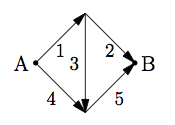
\includegraphics[width=\linewidth]{week6-control-1}
		\caption{}
		\label{fig:week6-control-1}
	\end{wrapfigure}

	Андрей владеет трубами 1 и 5; Борис владеет трубами 2 и 4; Володя владеет трубой 3.
	
	Пропускные способности труб: 3 - 1 литр/час, 1 и 4 - 2 литра в час, 2 и 5 - 3 литра/час.
	
	Потребители нефти готовы платить 1 рубль за каждый передаваемый литр/час.
	
	Сколько выигрывает коалиция Андрея и Володи?
	
	\textbf{Ответ:} 1

	\solution См. \hyperref[control:sol7]{\textit{ниже}}.
	
	\task
	Предположим, что $(x_1,\,x_2,\,x_3)$ -- дележ (Андрей, Борис, Володя) из ядра, причем $x_1=3$. Введите любое возможное значение $x_2$. Если таких дележей нет, введите $-1$.
	
	\textbf{Ответ:} 1
	
		\solution См. \hyperref[control:sol7]{\textit{ниже}}.
	
	\task
	
	Предположим, что $(x_1,\,x_2,\,x_3)$ -- дележ (Андрей, Борис, Володя) из ядра, причем $x_1=3$. Введите любое возможное значение $x_3$. Если таких дележей нет, введите $-1$.
	
	\textbf{Ответ:} 0
	
	\solution
	\label{control:sol7}
	
	Коалиция Андрея и Володи сможет пропусить только 1 литр в час по маршруту 1-3-5 (Володя больше не может пропустить по трубе 3).
	
	Найдем выигрыши коалиций. Каждый игрок по отдельности не получает ничего. Борис и Володя также не смогу получить ничего. Андрей и Борис могут прогнать 4 литра по своим трубам: 2 литра по маршруту 1-2 и 2 литра по маршруту 4-5. Все вместе также могут получить 4 литра. Условия на ядро:
	
	\[
	\left\{
		\begin{aligned}
			& x_1 + x_2 + x_3 = 4 \\
			& x_1 + x_2 \geq 4 \\
			& x_1 + x_2 \geq 1
		\end{aligned}
	\right.
	\]
	
	Легко понять, что $x_1 + x_2 = 4, \, x_3 = 0$. Значит, ядро состоит из дележей $(1+t,\, 3-t,\, 0)$, $t \in (0,\,3)$. Если $x_1 = 3$, то $x_2 = 1$, $x_3 = 0$.
	
	
\section{Вектор Шепли}

	\subsection{Тренировочные задачи}
	
	\task
	
	Рассмотрим игру ,,Продавцы и покупатели'' . Напомним правила игры.
	
	Имеется $M$ продавцов $a_1,\,a_2,\,\ldots\,,\,a_M$ и $N$ покупателей $b_1\,,\,b_2,\,\ldots\,,\,b_n$. У каждого продавца есть по 1 товару. Все товары одинаковы. Каждый из покупателей хочет приобрести 1 единицу товара. Если $m$ продавцов и $n$ покупателей встречаются, то их полезность равна количеству проданных единиц товара, то есть $\min(m,n)$.
	
	Рассмотрим неравенство $v(S \sqcup \{i\}) - v(S)\geq v(T \sqcup \{i\}) - v(T)$ для множеств игроков $T \subset S$ и $i \not \in S$.
	
	Отметьте те наборы $S,T,i$, при которых неравенство, указанное выше, выполнено:
	
	\begin{enumerate}[label=$\square$]
		\item[$\blacksquare$] $T = \left\{a_1,\, a_2\right\},\, S = \left\{a_1,\, a_2,\, a_3\right\},\, i = b_1$
		\item[$\blacksquare$] $T = \left\{a_1,\, a_2\right\},\, S = \left\{a_1,\,a_2,\,b_1\right\},\, i = b_2$
		\item $T=\left\{a_1\right\},\,S=\left\{a_1,\, b_1\right\},\, i = b_2$
		\item[$\blacksquare$] $T = \left\{a_1,\, b_1\right\},\, S = \left\{a_1,\, b_1,\, b_2\right\},\, i = a_2$
	\end{enumerate}

	\solution
	Поймём, когда при добавлении очередного игрока коалиция меняет свой выигрыш. Это происходит в том и только в том случае, когда при перед добавлением игрока количество игроков его "типа" (продавцов или покупателей) было строго меньше, чем игроков другого типа.
	
	Отсюда при добавлении покупателя $b_1$ коалиции $\{a_1,a_2\}$, $\{a_1,a_2,a_3\}$ выигрывают 1.
	
	Аналогично, при добавлении покупателя $b_2$ коалиции $\{a_1\}$, $\{a_1,a_2\}$, $\{a_1,a_2,b_1\}$ выигрывают 1, а коалиция $\{a_1,b_1\}$ не выигрывает ничего.
	
	При добавлении игрока $a_2$ коалиция $\{a_1,b_1\}$ не выигрывает ничего, а при добавлении к коалиции $\{a_1,b_1,b_2\}$ она выигрывает 1.
	
	\task
	Рассмотрим игру ,,Продавцы и покупатели'' . Напомним правила игры.
	
	Имеется $M$ продавцов $a_1,\,a_2,\,\ldots\,,\,a_M$ и $N$ покупателей $b_1\,,\,b_2,\,\ldots\,,\,b_n$. У каждого продавца есть по 1 товару. Все товары одинаковы. Каждый из покупателей хочет приобрести 1 единицу товара. Если $m$ продавцов и $n$ покупателей встречаются, то их полезность равна количеству проданных единиц товара, то есть $\min(m,n)$.
	
	Вектор Шепли является усреднением дележей, построенных по каждому из упорядочиваний игроков. Пусть $u_{\sigma}$ - это дележ, соответствующий упорядочиванию $\sigma$.
	
	При каких упорядочиваниях $\sigma$ продавец $B$ получит в дележе $u_\sigma$ выигрыш 1?
	
	\begin{enumerate}[label=$\square$]
		\item $\sigma = (B,\, 1,\, 2,\, 3,\, A)$
		\item[$\blacksquare$] $\sigma = (1,\, 2,\, 3,\, A,\, B)$
		\item $\sigma = (A,\, B,\, 1,\, 2,\, 3)$
		\item $\sigma = (3,\, A,\, B,\, 1,\, 2)$
		\item[$\blacksquare$] $\sigma = (2,\, 3,\, A,\, B,\, 1)$
	\end{enumerate}

	\solution
	% TODO: напиши решение
	
	\task
	Трое жителей: Аркадий, Борис и Василий, живут в соседних домиках. У каждого из них есть предпочтение в каком из домиков жить (эти предпочтения заданы в виде полезности). Несколько жителей могут договориться поменяться домиками для максимизации суммарной полезности. Предположим, что полезности заданы в виде следующей таблицы (по строчкам жители, а по столбцам домики):
	
	\begin{table}[h]
		\label{sheply:table1}
		\caption{}
		\centering
		\begin{tabular}{|c|c|c|c|}
			\hline & А & Б & В \\ 	
			\hline Аркадий & 2 & 4 & 7 \\ 
			\hline Борис & 3 & 2 & 1 \\ 
			\hline Василий & 5 & 4 & 4 \\ 
			\hline 
		\end{tabular} 
	\end{table}

	Формализуем данную игру как коалиционную (занумеруем игроков в алфавитном порядке). Рассмотрим вектор Шепли данной игры.
	
	Чему равна координата Аркадия в векторе Шепли?
	
	\textbf{Ответ:} $\frac{33}{6} = \frac{11}{2}$.
	
	\solution
	Используя решение задачи на прошлой \hyperref[arkadiy:sol1]{неделе}, построим таблицу дележей игроков в зависимости от упорядочивания:
	\begin{table}[h]
		\label{sheply:table2}
		\caption{}
		\centering
	\begin{tabular}{|c|c|c|c|}
		\hline 
		& Аркадий & Борис & Василий \\ 
		\hline 
		А, Б, В & 2 & 5 & 7 \\ 
		\hline 
		А, В, Б & 2 & 2 & 10 \\ 
		\hline 
		Б, А, В & 5 & 2 & 7 \\ 
		\hline 
		Б, В, А & 8 & 2 & 4 \\ 
		\hline 
		В, А, Б & 8 & 2 & 4 \\ 
		\hline 
		В, Б, А & 8 & 2 & 4 \\ 
		\hline 
		& 33 & 15 & 36 \\ 
		\hline 
	\end{tabular}
	\end{table}

	Отсюда Аркадий в векторе Шепли получит $\frac{33}{6} = \frac{11}{2}$, а Борис --- $\frac{15}{9}=\frac{5}{2}$.